\documentclass{beamer}
\usepackage{graphicx}
\usepackage{listings}

\lstdefinelanguage{Kotlin}{
comment=[l]{//},
commentstyle={\color{gray}\ttfamily},
emph={delegate, filter, first, firstOrNull, forEach, lazy, map, mapNotNull, println, return@},
emphstyle={\color{red}},
identifierstyle=\color{black},
keywords={abstract, actual, as, as?, break, by, class, companion, continue, data, do, dynamic, else, enum, expect, false, final, for, fun, get, if, import, in, interface, internal, is, null, object, operator, override, package, private, public, return, sealed, set, super, suspend, this, throw, true, try, typealias, val, var, vararg, when, where, while},
keywordstyle={\color{blue}\bfseries},
morecomment=[s]{/*}{*/},
morestring=[b]",
morestring=[s]{"""*}{*"""},
ndkeywords={@Deprecated, @JvmField, @JvmName, @JvmOverloads, @JvmStatic, @JvmSynthetic, Array, Byte, Double, Float, Int, Integer, Iterable, Long, Runnable, Short, String},
ndkeywordstyle={\color{Orange}\bfseries},
sensitive=true,
stringstyle={\color{green}\ttfamily},
showstringspaces=false,
}

\mode<presentation> { \usetheme{Madrid} }

\title{Kotlin\texorpdfstring{$\nabla$}{}}
\subtitle{Differentiable functional programming with algebraic data types}
\author{Breandan Considine}
\institute[UdeM]{
Universit\'e de Montr\'eal \\
\medskip
\textit{breandan.considine@umontreal.ca}
}
\date{\today}

\begin{document}
    \begin{frame}
        \titlepage
    \end{frame}

    \begin{frame}
        \frametitle{Overview}
        \tableofcontents
    \end{frame}

    \section{Introduction and motivation}\label{sec:first-section}

    %------------------------------------------------------------------------------------------------

    \begin{frame}
        \frametitle{Type checking automatic differentiation}
        Suppose we have a program $P: \mathbb{R}\rightarrow\mathbb{R}$ where:
        %
        \begin{equation}
            P(x)=p_n \circ p_{n-1} \circ p_{n-2} \circ ... \circ p_1 \circ p_0
        \end{equation}
        %
        From the chain rule of calculus, we know that:
        %
        \begin{equation}
            \frac{dP}{dp_0} = {\displaystyle \prod_{i=1}^{n} \frac{dp_{i}}{dp_{i-1}}}
        \end{equation}
        %
        In order for $P$ to type check, what is the type of $p_{0<i<n}$?
        \begin{equation}
            p_i: T_{out}(p_{i-1}) \rightarrow T_{in}(p_{i+1})
        \end{equation}
        %
        What happens if we let $P: \mathbb{R}^c\rightarrow\mathbb{R}$, $P: \mathbb{R}^c\rightarrow\mathbb{C}^d$  or $P: \Psi^p\rightarrow\Omega^q$?
    \end{frame}

    %------------------------------------------------------------------------------------------------

    \begin{frame}
        \frametitle{Why Kotlin?}
        \begin{itemize}
            \item Goal: To implement automatic differentiation in Kotlin
            \item Kotlin is a language with strong static typing and null safety
            \item Supports first-class functions, higher order functions and lambdas
            \item Has support for algebraic data types, via tuples & sealed classes
            \item Extension functions, operator overloading & other syntax sugar
            \item Offers features for embedding domain specific languages (DSLs)
            \item Access to all libraries and frameworks in the JVM ecosystem
            \item Multi-platform and cross-platform (JVM, Android, iOS, JS, native)
        \end{itemize}
        \begin{center}
            
\includegraphics[scale=0.05]{kotlin.png}
        \end{center}
    \end{frame}

    \begin{frame}
        \frametitle{Kotlin\texorpdfstring{$\nabla$}{} Priorities}
        \begin{itemize}
            \item Type system requirements
            \begin{itemize}
                \item Strong type system based on algebraic principles
                \item Leverage the compiler for static analysis
                \item No implicit broadcasting or shape coercion
                \item Parameterized numerical types and arbitary-precision
            \end{itemize}
            \item Design principles
            \begin{itemize}
                \item Functional programming and lazy numerical evaluation
                \item Eager algebraic simplification of expression trees
                \item Operator overloading and tapeless reverse mode AD
            \end{itemize}
            \item Usage desirata
            \begin{itemize}
                \item Generalized AD with imperative array programming
                \item Automatic differentiation with infix and Polish notation
                \item Partials and higher order derivatives and gradients
            \end{itemize}
            \item Testing and validation
            \begin{itemize}
                \item Numerical gradient checking and property-based testing
                \item Performance benchmarks and thorough regression testing
            \end{itemize}
        \end{itemize}
    \end{frame}

    \begin{frame}
        \frametitle{Algebraic types}
        \begin{itemize}
            \item Abstract algebra can be useful when generalizing to new structures
            \item Helps us to easily translate between mathematics and code
            \item Most of the time in numerical computing, we are dealing with Fields
            \begin{itemize}
                \item A set $F$ together with two operations $+$ and $\times$
                \begin{itemize}
                    \item Associativity: $\forall a, b, c \in F, a + (b + c) = (a + b) + c$
                    \item Commutivity: $\forall a, b \in F, a + b = b + a$ and $a\times b = b\times a$
                    \item Distributivity: $\forall a, b, c \in F, a \times (b \times c) = (a \times b) \times c$
                    \item Identity: $\forall a \in F, \exists 0$, $ 1 \in F$ s.t. $a + 0 = a$ and $a\times 1= a$
                    \item $+$ inverse: $\forall a\in F, \exists -a$ s.t. $a + (-a) = 0$
                    \item $\times$ inverse: $\forall a\neq 0 \in F, \exists a^{-1}$ s.t. $a \times a^{-1} = 1$
                \end{itemize}
            \end{itemize}
            \item Readily extensible to complex numbers, quaternions, dual numbers
            \item Can be implemented using parametric polymorphism a.k.a. generics
        \end{itemize}
    \end{frame}


    \begin{frame}[fragile]
        \frametitle{How do we define algebraic types in Kotlin\texorpdfstring{$\nabla$}{}?}
        \begin{lstlisting}[language=Kotlin, gobble=12]
            // T: Group<T> is effectively a self type
            interface Group<T: Group<T>> {
              operator fun plus(f: T): T
              operator fun times(f: T): T
            }

            // Inherits from Group, default methods
            interface Field<T: Field<T>>: Group<T> {
              operator fun unaryMinus(): T
              operator fun minus(f: T): T = this + -f
              fun inverse(): T
              operator fun div(f: T): T = this * f.inverse()
            }
        \end{lstlisting}
    \end{frame}

    %    \section{A Short History of Computing Derivatives}\label{sec:second-section}
    %
    %    \begin{frame}
    %        \frametitle{Numerical differentiation}
    %        \begin{itemize}
    %            \item Many mathematical formula have discrete, numerical representations
    %            \item But numerical values can be an \textit{inexact} representation of math
    %            \item Long calculations on primitives are susceptible to rounding errors
    %            \item Bag of tricks for discrete approximation and numerical stability:
    %            \begin{itemize}
    %                \item Fourier, Chebyshev, Lagrange
    %                \item Arbitrary precision arithmetic
    %                \item Kahan summation algorithm
    %                \item log-sum-exp trick
    %            \end{itemize}
    %        \end{itemize}
    %    \end{frame}

    %------------------------------------------------------------------------------------------------

    %    \begin{frame}
    %        \frametitle{Symbolic differentiation}
    %        \begin{itemize}
    %            \item What about evaluating functions symbolically?
    %            \item Computer algebra systems for manipulate symbolic formulas
    %        \end{itemize}
    %    \end{frame}

    %------------------------------------------------------------------------------------------------

    %    \begin{frame}
    %        \frametitle{Automatic differentiation}
    %        \begin{itemize}
    %            \item Derivatives can be calculated automatically? (Wengert, 1964)
    %            \item Code as an \textit{exact} symbolic representation of functions
    %            \item To reason about code we need the ability to treat \textit{code as data}:
    %            \begin{itemize}
    %                \item Reflection and metaprogramming
    %                \item Domain specific languages
    %                \item First-class functions
    %            \end{itemize}
    %        \end{itemize}
    %    \end{frame}

    %------------------------------------------------------------------------------------------------

    %    \begin{frame}
    %        \frametitle{Differentiable [functional] programming}
    %        \begin{itemize}
    %            \item What is a program, but a series of arithmetic operations?
    %            \item What are arithmetic operations but syntactic sugar for functions?
    %            \item Functions can be composed of other functions or chained in sequence
    %            \item High school calculus gives us rules for differentiating function chains
    %            \item Pearlmutter \& Siskind teach us AD is possible just using FP (2016)
    %            \item Wang, Rompf, et al. show us this is possible \textit{without a tape}! (2018)
    %        \end{itemize}
    %    \end{frame}

    %------------------------------------------------------------------------------------------------

    %    \begin{frame}
    %        \frametitle{Differentiable programming with algebraic types}
    %        \begin{itemize}
    %            \item Combine the tools from mathematics and CS
    %            \item Type safety
    %            \item Static analysis
    %            \item Allows us to preserve symmetries that are not obvious
    %            \item There is an abstract algebra for tensor manipulations
    %            \item Can be encoded using OOP and parametric polymorphism
    %            \item \href{https://arxiv.org/pdf/1610.07690.pdf}{Operational Calculus for Differentiable Programming}
    %        \end{itemize}
    %    \end{frame}

    %------------------------------------------------------------------------------------------------

    \section{Architectural Overview}\label{sec:third-section}

    \begin{frame}[fragile]
        \frametitle{Algebraic Data Types}
        \begin{lstlisting}[language=Kotlin, gobble=12]
            class Var: Expr()
            class Const(val num: Number): Expr()
            class Sum(val e1: Expr, val e2: Expr): Expr()
            class Prod(val e1: Expr, val e2: Expr): Expr()
            sealed class Expr: Group {
              fun diff() = when(expr) {
                is Const -> Zero
                is Sum -> e1.diff() + e2.diff()
                // d(u*v)/dx = du/dx * v + u * dv/dx
                is Prod -> e1.diff() * e2 + e1 * e2.diff()
                is Var -> One
              }
              operator fun plus(e: Expr) = Sum(this, e)
              operator fun times(e: Expr) = Prod(this, e)
            }
        \end{lstlisting}
    \end{frame}

    \begin{frame}[fragile]
        \frametitle{Expression Simplification}
        \begin{lstlisting}[language=Kotlin, gobble=12]
            operator fun Expr.times(exp: Expr) = when {
              this is Const && num == 0.0 -> Const(0.0)
              this is Const && num == 1.0 -> exp
              exp is Const && exp.num == 0.0 -> exp
              exp is Const && exp.num == 1.0 -> this
              this is Const && exp is Const -> Const(num*exp.num)
              else -> Prod(this, e)
            }

            // Sum(Prod(Const(2.0), Var()), Const(6.0))
            val q = Const(2.0) * Sum(Var(), Const(3.0))
        \end{lstlisting}
    \end{frame}

    \begin{frame}[fragile]
        \frametitle{Testing}
        \begin{lstlisting}[language=Kotlin, gobble=12]
            val x = variable("x")
            val y = variable("y")

            val z = y * (sin(x * y) - x) // Function under test
            val dz_dx = d(z) / d(x)      // Automatic derivative
            val manualDx = y * (cos(x * y) * y - 1)

            "dz/dx should be y * (cos(x * y) * y - 1)" {
              assertAll (NumGen, NumGen) { cx, cy ->
                // Evaluate the results at a given seed
                val autoEval = dz_dx(x to cx, y to cy)
                val manualEval = manualDx(x to cx, y to cy)
                // Should pass if |adEval - manualEval| < eps
                autoEval shouldBeApproximately manualEval
              }
            }
        \end{lstlisting}
    \end{frame}

    \section{Usage}\label{sec:fourth-section}

    \begin{frame}[fragile]
        \frametitle{Usage}
        \begin{lstlisting}[language=Kotlin, gobble=12]
            with(DoubleFunctor) {// Use double-precision numerics
             val x = variable()  // Declare an immutable variable
             val y = sin(sin(sin(x)))/x + sin(x) * x + cos(x) + x

             // Lazily compute reverse-mode automatic derivatives
             val dy_dx = d(y) / d(x)
             val d2y_dx = d(dy_dx) / d(x)
             val d3y_dx = d(d2y_dx2) / d(x)
             val d4y_dx = d(d3y_dx3) / d(x)
             val d5y_dx = d(d4y_dx4) / d(x)

             plot(-10..10, dy_dx, dy2_dx, d3y_dx, d4y_dx, d5y_dx)
            }
        \end{lstlisting}
    \end{frame}

    \begin{frame}
        \frametitle{$y = \frac{\sin{\sin{\sin{x}}}}{x} + x \sin{x} + \cos{x} + x$, $\frac{dy}{dx}$, $\frac{d^{2}y}{dx^2}$, $\frac{d^{3}y}{dx^3}$, $\frac{d^{4}y}{dx^4}$, $\frac{d^{5}y}{dx^5}$}
        \begin{center}
            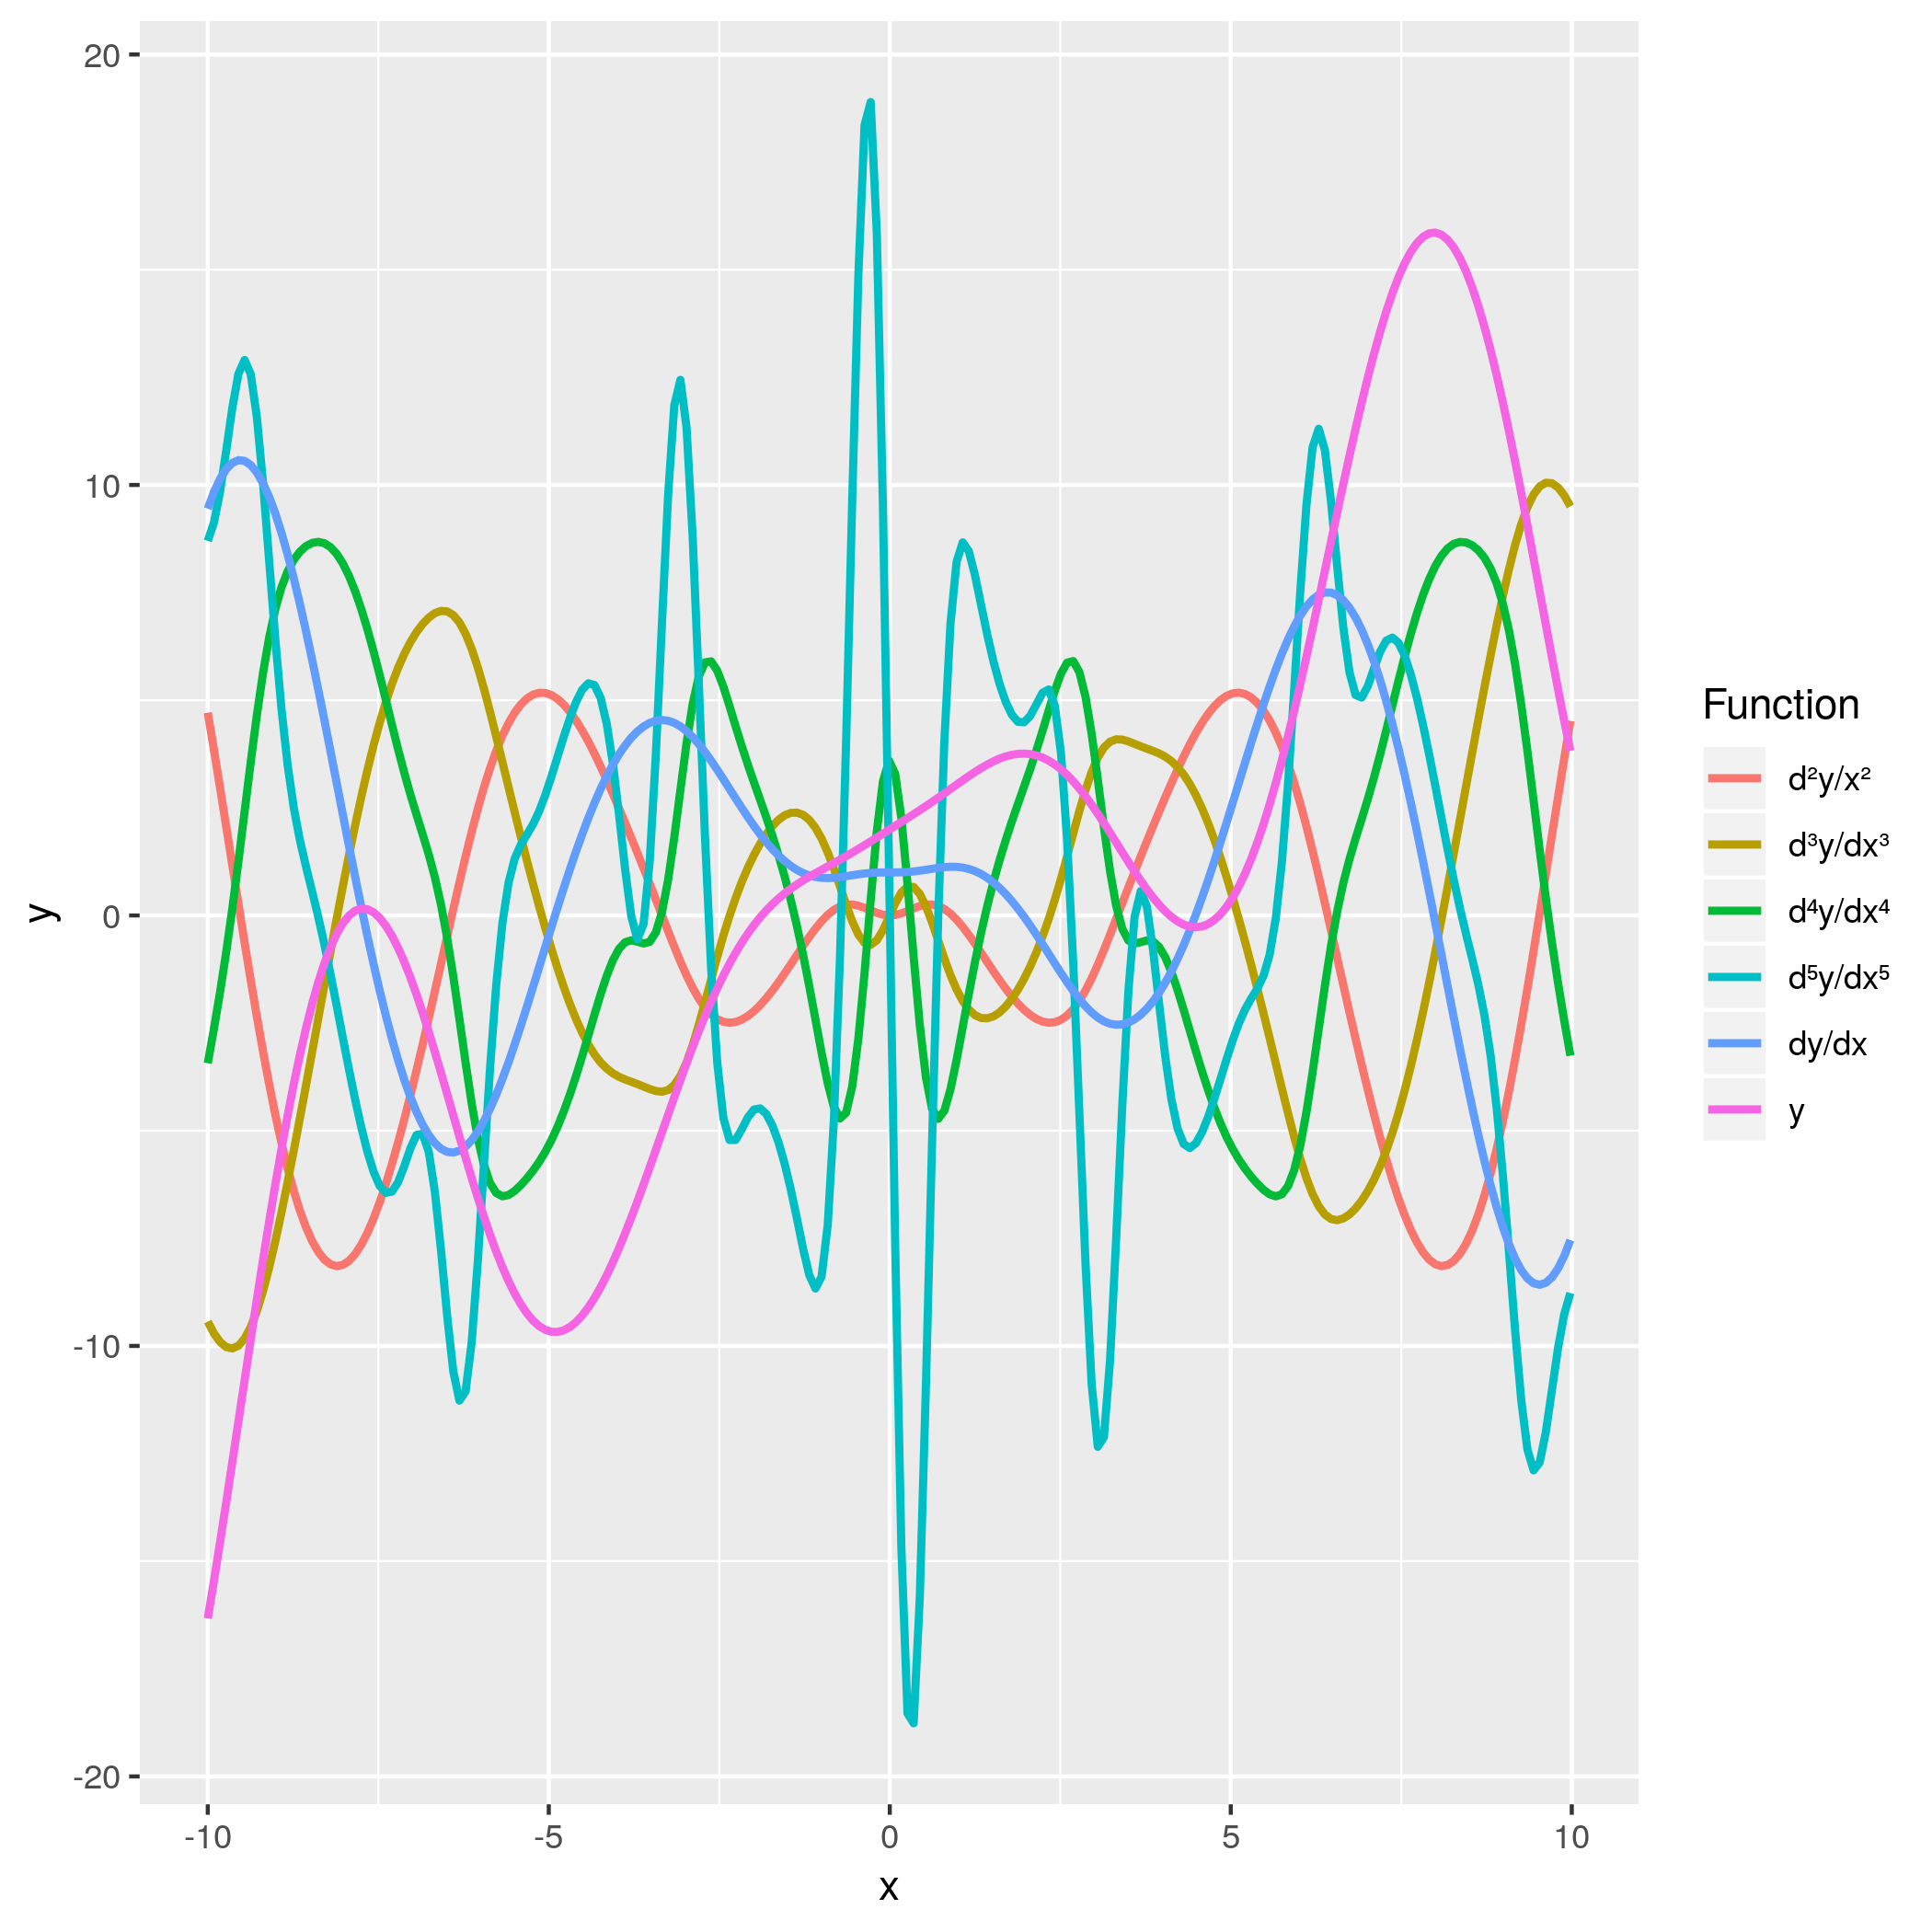
\includegraphics[scale=0.4]{plot.png}
        \end{center}
    \end{frame}

    \section{Future Plans}\label{sec:fifth-section}

    \begin{frame}
        \frametitle{Further directions to explore}
        \begin{itemize}
            \item Closer integration with Kotlin/Java standard library
            \item \href{https://discuss.kotlinlang.org/t/primitive-type-specialization/11022/4}{Primitive type specialization}
            \item Dependent types via code generation to type check tensor shapes
            \item Encode additional structure like function arity into type system
            \item Performance benchmarks and zero-cost un/boxing abstractions
            \item Configurable forward and backward AD modes
            \item Automatic expression refactoring for numerical stability
        \end{itemize}
    \end{frame}

    \begin{frame}
        \begin{center}
            \Huge{Learn more at: \\
            kg.ndan.co}
        \end{center}
    \end{frame}

    \begin{frame}
        \frametitle{Special thanks}
        \begin{itemize}
            \begin{center}
                \huge{
                Liam Paull \\
                Michalis Famelis \\
                Alexander Nozik \\
                Hanneli Tavante \\~\\
                }
                
\includegraphics[scale=0.1]{udem.png}
                
\includegraphics[scale=0.4]{mila.png}
            \end{center}
        \end{itemize}
    \end{frame}
\end{document}